\documentclass[10pt]{article}
\usepackage[a4paper, total={6in,9in}]{geometry}
\usepackage[parfill]{parskip}    	
\usepackage{graphicx,caption,fancyhdr,xcolor,pdfpages,setspace}
\usepackage{minted}
\usepackage{xcolor}
\usepackage[
        colorlinks = true,
        allcolors  = darkgray
]{hyperref}



\newcommand{\wrt}[1]{\mathrm{d}#1}


\setlength{\fboxsep}{0.5em}



\urlstyle{same}
\renewcommand{\footnoterule} % Push footnotes to the bottom of the pagehttps://www.overleaf.com/project/634eca5f6262ed6dd715c645
	{\vfill\kern -3pt \hrule width 0.4\columnwidth \kern 2.6pt}

\makeatletter
\title{Digital Design with HDL Lab 4}
\let\Title\@title
\author{Y3862181 \& Y3899129}
\let\Author\@author
\date{Summer Term, 2022}
\let\Date\@date
\makeatother


\fancypagestyle{content}{
    \renewcommand{\headrulewidth}{0.4pt}
    \renewcommand{\footrulewidth}{0.4pt}
    \setlength{\headheight}{15pt}
    
	\fancyhf{}
	\fancyhead[L]{\Author}
	\fancyhead[R]{\Title}
	\fancyfoot[L]{\Date}
	\fancyfoot[R]{\thepage}
}
\onehalfspacing
\begin{document}
\begin{titlepage}
\centering
{\Huge Lab Report 4}

\vspace{3cm}

{\LARGE \textbf{ Digital Design with HDL}}

\vspace{3cm}

{\huge Y3862181 \& Y3899129}

\vspace{3cm}


{\large Autumn Term, 2022}
\vfill

{\itshape University of York}
\end{titlepage}

\tableofcontents
\newpage

\pagestyle{content}
\section{Introduction}

In this lab, both a parameterizable ALU and Shift Register will be implemented and tested in VHDL using self-checking testbenches. In addition to the required specifications, a human-readable self-checking testbench procedure for the parameterizable ALU will be utilised in order to minimise any potential errors that could occur when setting up any test vectors.    

\newpage

\section{Task A: A parameterizable ALU}
\subsection{Parameterizable ALU Design \texttt{(par\_alu.vhd)}}
\begin{minted}{vhdl}
library IEEE;
use IEEE.STD_LOGIC_1164.ALL;
use IEEE.NUMERIC_STD.ALL;

-- Custom library containing defined functions for log2() and
-- definitions of the constants for the opcodes
use work.DigEng.all;

-- Implementation of ALU with parametrizable data size
-- Supported operations: Identity, AND, OR, XOR, NOT, Addition, Subtraction, 
-- Incrementation, Decrementation, Arithmetic shift left, 
-- Arithmetic shift right, Rotation left and Rotation right
-- Also it supports flags for: equal to zero, not equal to zero, equal to one, 
-- less than zero, higher than zero, less or equal to zero, 
-- higher or equal to zero and an overflow

entity par_alu is
    -- The width of the data busses (inputs and outputs) with 8-bits being 
    -- the default value
    Generic (data_size : integer := 8);
    Port ( A       : in  STD_LOGIC_VECTOR (data_size - 1 downto 0);
           B       : in  STD_LOGIC_VECTOR (data_size - 1 downto 0);
           -- Number of bits with which the data should be shifted or rotated
           X       : in  STD_LOGIC_VECTOR (log2(data_size)-1 downto 0);
           OPCODE  : in  STD_LOGIC_VECTOR (3 downto 0);
           ALU_OUT : out STD_LOGIC_VECTOR (data_size - 1 downto 0);
           FLAGS   : out STD_LOGIC_VECTOR (7 downto 0));
end par_alu;

architecture Behavioral of par_alu is

-- Internal bus for the output of the ALU
-- It is used so the output of the ALU can be accessed from the vhdl code 
-- and used to generate the flags
signal alu_out_internal : STD_LOGIC_VECTOR (data_size - 1 downto 0);

-- Internal busses to hold the values for the different operations
signal val_incr    : STD_LOGIC_VECTOR (data_size - 1 downto 0);
signal val_decr    : STD_LOGIC_VECTOR (data_size - 1 downto 0);
signal val_sum     : STD_LOGIC_VECTOR (data_size - 1 downto 0);
signal val_diff    : STD_LOGIC_VECTOR (data_size - 1 downto 0);
signal val_shift_l : STD_LOGIC_VECTOR (data_size - 1 downto 0);
signal val_shift_r : STD_LOGIC_VECTOR (data_size - 1 downto 0);
signal val_rot_l   : STD_LOGIC_VECTOR (data_size - 1 downto 0);
signal val_rot_r   : STD_LOGIC_VECTOR (data_size - 1 downto 0);

-- Internal signals to hold the signs of input A, input B, and the ALU output
-- 0 = positive, 1 = negative
signal sign_a       : STD_LOGIC;
signal sign_b       : STD_LOGIC;
signal sign_alu_out : STD_LOGIC;

begin

-- Assign the arithmetic operations to their coresponding variables
val_incr <= std_logic_vector ( signed(A) + 1 );
val_decr <= std_logic_vector ( signed(A) - 1 );
val_sum  <= std_logic_vector ( signed(A) + signed(B) );
val_diff <= std_logic_vector ( signed(A) - signed(B) );

-- Assign the shift operations to their coresponding variables
val_shift_l <= std_logic_vector(shift_left(signed(A), to_integer(unsigned(X))));
val_shift_r <= std_logic_vector(shift_right(signed(A), to_integer(unsigned(X))));
val_rot_l <= std_logic_vector(rotate_left(signed(A), to_integer(unsigned(X))));
val_rot_r <= std_logic_vector(rotate_right( signed(A), to_integer(unsigned(X))));

-- Map the output bus to the coresponding operation for the selected opcode
alu_out_internal <= ( A           ) when OPCODE = OP_IDENTITY else
                    ( A AND B     ) when OPCODE = OP_AND      else
                    ( A OR B      ) when OPCODE = OP_OR       else
                    ( A XOR B     ) when OPCODE = OP_XOR      else
                    ( NOT A       ) when OPCODE = OP_NOT      else
                    ( val_incr    ) when OPCODE = OP_INCR     else
                    ( val_decr    ) when OPCODE = OP_DECR     else
                    ( val_sum     ) when OPCODE = OP_SUM      else
                    ( val_diff    ) when OPCODE = OP_DIFF     else
                    ( val_shift_l ) when OPCODE = OP_SHIFT_L  else
                    ( val_shift_r ) when OPCODE = OP_SHIFT_R  else
                    ( val_rot_l   ) when OPCODE = OP_ROT_L    else
                    ( val_rot_r   ) when OPCODE = OP_ROT_R    else
                    (others => '0'); 


-- Assign the output of the ALU to the internal bus holding the value.
ALU_OUT <= alu_out_internal;

--------------------------------------------------
-- Flag assignments
--------------------------------------------------

-- When the output is zero
FLAGS(0) <= '1' when signed(alu_out_internal) = 0  else '0';

-- When the output is not zero
FLAGS(1) <= '0' when signed(alu_out_internal) = 0  else '1';

-- When the output is one
FLAGS(2) <= '1' when signed(alu_out_internal) = 1  else '0';

-- When the output is less than zero
FLAGS(3) <= '1' when signed(alu_out_internal) < 0  else '0';

-- When the output is higher than zero
FLAGS(4) <= '1' when signed(alu_out_internal) > 0  else '0';

-- When the output is less or equal to zero
FLAGS(5) <= '1' when signed(alu_out_internal) <= 0 else '0';

-- When the output is higher or equal to zero
FLAGS(6) <= '1' when signed(alu_out_internal) >= 0 else '0';        


-- Overflow Flag Implementation

-- Extract the sign of the number held in A in 
-- sign_a ( 0 = positive, 1 = negative ) 
sign_a <= A(data_size-1);

-- Extract the sign of variable B when the opcode is Summation
-- Extract and invert the sign of B when the opcode is Difference
-- Assign negative sign for B when the operation is Decrement
-- Assign positive sign for B when the operation is Increment
sign_b <= '1' when ( (signed(B) < 0)       and (OPCODE = OP_SUM )) or
                   ( not ( signed(B) < 0 ) and (OPCODE = OP_DIFF)) or
                   ( OPCODE = OP_DECR    )
              else '0'; -- positive when the opcode is Increment

-- Extract the sign of the output of the ALU (0 = positive, 1 = negative)
sign_alu_out <= '1' when signed(alu_out_internal) < 0 else '0';

-- The ALU overflows when the two input numbers signs are identical 
-- (sign_a, sign_b) and the sign of the output is different
-- The overflow flag is used only with arithmetic operations, 
-- hence ( OPCODE(3) = '1' and OPCODE(2) = '0')
FLAGS(7)     <= (sign_a xnor sign_b) and (sign_a xor sign_alu_out) 
                when (OPCODE(3) = '1' and OPCODE(2) = '0') else '0';

end Behavioral;


\end{minted}
\newpage
\subsection{Supporting Library for the ALU and the Testbenches \texttt{(Dig\_Eng.vhd)}}
\begin{minted}{vhdl}
----------------------------------------------------
-- PACKAGE FOR DIGITAL ENGINEERING LABS
--
-- To use:
--
-- - Download file
-- - Use "Add copy" to add to Xilinx project
-- - Add "use work.DigEng.all" on top of entity
--
----------------------------------------------------
library IEEE;
use IEEE.STD_LOGIC_1164.ALL;
use IEEE.NUMERIC_STD.ALL;

-- Library for string related functions
use std.textio.all;


package DigEng is

function log2 (x : natural ) return natural;
function size (x : natural ) return natural;

-- Definitions of the operators constants
constant OP_IDENTITY : STD_LOGIC_VECTOR  (3 downto 0) := "0000";

constant OP_AND     : STD_LOGIC_VECTOR  (3 downto 0) := "0100";
constant OP_OR      : STD_LOGIC_VECTOR  (3 downto 0) := "0101";
constant OP_XOR     : STD_LOGIC_VECTOR  (3 downto 0) := "0110";
constant OP_NOT     : STD_LOGIC_VECTOR  (3 downto 0) := "0111";

constant OP_INCR    : STD_LOGIC_VECTOR  (3 downto 0) := "1000";
constant OP_DECR    : STD_LOGIC_VECTOR  (3 downto 0) := "1001";
constant OP_SUM     : STD_LOGIC_VECTOR  (3 downto 0) := "1010";
constant OP_DIFF    : STD_LOGIC_VECTOR  (3 downto 0) := "1011";

constant OP_SHIFT_L : STD_LOGIC_VECTOR  (3 downto 0) := "1100";
constant OP_SHIFT_R : STD_LOGIC_VECTOR  (3 downto 0) := "1101";
constant OP_ROT_L   : STD_LOGIC_VECTOR  (3 downto 0) := "1110";
constant OP_ROT_R   : STD_LOGIC_VECTOR  (3 downto 0) := "1111";


-- Test vector type definition
type test_vector_t is record
    OPCODE  : STD_LOGIC_VECTOR (3 downto 0); 
    A       : STD_LOGIC_VECTOR (15 downto 0);
    B       : STD_LOGIC_VECTOR (15 downto 0);
    X       : STD_LOGIC_VECTOR (3 downto 0);
    ALU_OUT : STD_LOGIC_VECTOR (15 downto 0);
    FLAGS   : STD_LOGIC_VECTOR (7 downto 0);
end record;

----------------------------------------------------
-- FUNCTION TO ASSEMBLE A TEST VECTOR GIVEN DECIMAL VALUES
----------------------------------------------------
function to_test_vector_d (
    OPCODE  : STD_LOGIC_VECTOR (3 downto 0);
    A : integer;
    B : integer;
    X : integer;
    ALU_OUT: integer;
    FLAGS   : STD_LOGIC_VECTOR (7 downto 0)
) return test_vector_t;

----------------------------------------------------
-- FUNCTION TO ASSEMBLE A TEST VECTOR GIVEN BINARY VALUES
----------------------------------------------------
function to_test_vector_b (
    OPCODE  : STD_LOGIC_VECTOR (3 downto 0);
    A : STD_LOGIC_VECTOR (15 downto 0);
    B : STD_LOGIC_VECTOR (15 downto 0);
    X : integer;
    ALU_OUT: STD_LOGIC_VECTOR (15 downto 0);
    FLAGS   : STD_LOGIC_VECTOR (7 downto 0)
) return test_vector_t;

----------------------------------------------------
-- INTEGER TO STD_LOGIC_VECTOR OF WIDTH 16
----------------------------------------------------
function int_to_std16 (
    x : integer 
) return std_logic_vector;



----------------------------------------------------
-- RETURNS A STRING WITH THE NAME OF THE GIVEN OPCODE
----------------------------------------------------
function opcode_to_str (
    OPCODE  : STD_LOGIC_VECTOR (3 downto 0)
) return string;

----------------------------------------------------
-- RETURN A STRING WITH AN ERROR MESSAGE FOR A SPECIFIC TEST VECTOR
----------------------------------------------------
function test_vector_to_err_str (
    ID: INTEGER;
    TEST_VECTOR: test_vector_t;
    ALU_OUT: STD_LOGIC_VECTOR (15 downto 0);
    FLAGS: STD_LOGIC_VECTOR (7 downto 0)
) return string;

end DigEng;

























package body DigEng is

----------------------------------------------------
-- LOG BASE 2 FUNCTION
-- returns the ceiling of log base 2 of a (non-zero) integer
-- (1->0; 2->1; 3->2; 4->2; 5->3 ...)
--
-- This function is NOT SYNTHESIZABLE 
-- should be used for indices, not circuit description
-- 
-- Examples:
-- - signal A : STD_LOGIC_VECTOR(log2(data_size)-1 downto 0);
-- 
----------------------------------------------------
function log2 ( x : natural ) return natural is
        variable temp : natural := x ;
        variable n : natural := 0 ;
    begin
        while temp > 1 loop
            temp := temp / 2 ;
            n := n + 1 ;
        end loop ;
	   if (x > 2**n) then
		n := n + 1;
	   end if;
        return n ;
end function log2;
















----------------------------------------------------
-- SIZE FUNCTION
-- returns the size of a vector that can encode a (non-zero) integer
-- (1->1; 2->2; 3->2; 4->3; 5->3 ...)
--
-- This function is NOT SYNTHESIZABLE 
-- should be used for indices, not circuit description
-- 
-- Examples:
-- - signal A : STD_LOGIC_VECTOR(size(n)-1 downto 0);
-- 
----------------------------------------------------
function size ( x : natural ) return natural is
        variable temp : natural := x ;
        variable n : natural := 0 ;
    begin
        while temp >= 1 loop
            temp := temp / 2 ;
            n := n + 1 ;
        end loop ;
        return n ;
end function size;





















----------------------------------------------------
-- FUNCTION TO ASSEMBLE A TEST VECTOR GIVEN DECIMAL VALUES
-- 
-- The decimal values apply only for the A, B, X and ALU_OUT.
-- The other parameters: OPCODE and FLAGS are STD_LOGIC_VECTORS
-- of 4 and 8 bits respectively.
--
-- Return: test_vector_t
----------------------------------------------------
function to_test_vector_d (
    OPCODE  : STD_LOGIC_VECTOR (3 downto 0);
    A : integer;
    B : integer;
    X : integer;
    ALU_OUT: integer;
    FLAGS   : STD_LOGIC_VECTOR (7 downto 0)
) return test_vector_t is
    variable TEST_VECTOR: test_vector_t;
begin
    TEST_VECTOR.OPCODE := OPCODE;
    TEST_VECTOR.A := int_to_std16(A);
    TEST_VECTOR.B := int_to_std16(B);
    TEST_VECTOR.X := std_logic_vector(to_unsigned(X,4));
    TEST_VECTOR.ALU_OUT := int_to_std16(ALU_OUT);
    TEST_VECTOR.FLAGS := FLAGS;
    
    return TEST_VECTOR;

end function to_test_vector_d;














----------------------------------------------------
-- FUNCTION TO ASSEMBLE A TEST VECTOR GIVEN BINARY VALUES
-- 
-- The binary values apply only for the A, B and ALU_OUT.
-- The other parameters: OPCODE and FLAGS are STD_LOGIC_VECTORS
-- of 4 and 8 bits respectively, and X is an integer
--
-- Return: test_vector_t
----------------------------------------------------
function to_test_vector_b (
    OPCODE  : STD_LOGIC_VECTOR (3 downto 0);
    A : STD_LOGIC_VECTOR (15 downto 0);
    B : STD_LOGIC_VECTOR (15 downto 0);
    X : integer;
    ALU_OUT: STD_LOGIC_VECTOR (15 downto 0);
    FLAGS   : STD_LOGIC_VECTOR (7 downto 0)
) return test_vector_t is
    variable TEST_VECTOR: test_vector_t;
begin
    TEST_VECTOR.OPCODE := OPCODE;
    TEST_VECTOR.A := A;
    TEST_VECTOR.B := B;
    TEST_VECTOR.X := std_logic_vector(to_unsigned(X,4));
    TEST_VECTOR.ALU_OUT := ALU_OUT;
    TEST_VECTOR.FLAGS := FLAGS;
    
    return TEST_VECTOR;

end function to_test_vector_b;

----------------------------------------------------
-- INTEGER TO STD_LOGIC_VECTOR OF WIDTH 16
--
-- Input: integer
-- Output: STD_LOGIC_VECTOR (15 downto 0)
----------------------------------------------------
function int_to_std16 ( 
    x : integer 
) return std_logic_vector is
begin
   return std_logic_vector(to_signed(x,16));
end function int_to_std16;

----------------------------------------------------
-- RETURNS A STRING WITH THE NAME OF THE GIVEN OPCODE
--
-- Input: STD_LOGIC_VECTOR (3 downto 0)
-- Output: string
----------------------------------------------------
function opcode_to_str (
    OPCODE  : STD_LOGIC_VECTOR (3 downto 0)
) return string is
begin
    if (OPCODE = OP_IDENTITY) then
        return string'("OP_IDENTITY");
    elsif (OPCODE = OP_AND) then
        return string'("OP_AND");
    elsif (OPCODE = OP_OR) then
        return string'("OP_OR");
    elsif (OPCODE = OP_XOR) then
        return string'("OP_XOR");
    elsif (OPCODE = OP_NOT) then
        return string'("OP_NOT");
    elsif (OPCODE = OP_INCR) then
        return string'("OP_INCR");
    elsif (OPCODE = OP_DECR) then
        return string'("OP_DECR");
    elsif (OPCODE = OP_SUM) then
        return string'("OP_SUM");
    elsif (OPCODE = OP_DIFF) then
        return string'("OP_DIFF");
    elsif (OPCODE = OP_SHIFT_L) then
        return string'("OP_SHIFT_L");
    elsif (OPCODE = OP_SHIFT_R) then
        return string'("OP_SHIFT_R");
    elsif (OPCODE = OP_ROT_L) then
        return string'("OP_ROT_L");
    elsif (OPCODE = OP_ROT_R) then
        return string'("OP_ROT_R");
    end if;
end function opcode_to_str;





----------------------------------------------------
-- RETURN A STRING WITH AN ERROR MESSAGE FOR A SPECIFIC TEST VECTOR
--
-- Inputs: ID: integer (The number of the test vector)
--         TEST_VECTOR: test_vector_t (the test vector 
--                      with the inputs and the expected outputs)
--         ALU_OUT: STD_LOGIC_VECTOR (15 downto 0) (The generated ALU_OUT)
--         FLAGS: STD_LOGIC_VECTOR (7 downto 0) (The generated FLAGS)
----------------------------------------------------
function test_vector_to_err_str (
    ID: INTEGER;
    TEST_VECTOR: test_vector_t;
    ALU_OUT: STD_LOGIC_VECTOR (15 downto 0);
    FLAGS: STD_LOGIC_VECTOR (7 downto 0)
) return string is
    -- Variable to hold the error message
    variable err_msg: line := new string'("");
    
    -- Temporary variable to hold the value of a single bit of the flags
    -- used to generate the binary print
    variable flag_tmp: integer;
begin
    -- The write function resizes the output string and 
    -- copies the data into the newely realocated string
    write(err_msg, string'("[Test vector "));
    write(err_msg, string'(integer'image(ID)));
    write(err_msg, string'(" Failed] inputs: ["));
    write(err_msg, opcode_to_str(TEST_VECTOR.OPCODE));
    write(err_msg, string'(" A = "));
    write(err_msg, string'(integer'image(to_integer(signed(TEST_VECTOR.A)))));
    write(err_msg, string'(" B = "));
    write(err_msg, string'(integer'image(to_integer(signed(TEST_VECTOR.B)))));
    write(err_msg, string'(" X = "));
    write(err_msg, string'(integer'image(to_integer(unsigned(TEST_VECTOR.X)))));
    write(err_msg, string'("] outputs: [ALU_OUT = "));
    write(err_msg, string'(integer'image(to_integer(signed(ALU_OUT)))));
    write(err_msg, string'(" expected "));
    write(err_msg, string'(integer'image(to_integer(signed(TEST_VECTOR.ALU_OUT)))));
    write(err_msg, string'("], [FLAGS = "));
    
    
    
    
    -- Loop to look through each flag and add it to the err_msg
    for i in 0 to 7 loop
        flag_tmp := to_integer(unsigned'('0' & FLAGS(7-i)));
        write(err_msg, string'(integer'image( flag_tmp )));
    end loop;
    
    write(err_msg, string'(" expected "));
    
    -- Loop to look through each flag and add it to the err_msg
    for i in 0 to 7 loop
        flag_tmp := to_integer(unsigned'('0' & TEST_VECTOR.FLAGS(7-i)));
        write(err_msg, string'(integer'image( flag_tmp )));
    end loop;
    
    write(err_msg, string'("]"));
    
    -- Finally return the fully assembled string (err_msg)
    return err_msg.all;
end function test_vector_to_err_str;


end DigEng;
\end{minted}
\newpage


\subsection{Self-checking ALU Testbench \texttt{(par\_alu\_tb.vhd)}}
\begin{minted}{vhdl}
library IEEE;
use IEEE.STD_LOGIC_1164.ALL;
use IEEE.NUMERIC_STD.ALL;

-- Custom library containing definitions for:
-- test_vector_t type, to_test_vector_d(), 
-- to_test_vector_b() amd print_test_vector()
use work.DigEng.all;

-- Test bench to confirm the correct operation of the parametrizable ALU 
-- using a self checking test bench.
-- For 16-bit data size


entity par_alu_tb is
end par_alu_tb;

architecture Behavioral of par_alu_tb is

-- Internal signals that connect to the inputs and outputs of the ALU
signal A       : STD_LOGIC_VECTOR (15 downto 0);
signal B       : STD_LOGIC_VECTOR (15 downto 0);
-- (X) Number of bits with which the data should be shifted or rotated
signal X       : STD_LOGIC_VECTOR (3 downto 0); 
signal OPCODE  : STD_LOGIC_VECTOR (3 downto 0);
signal ALU_OUT : STD_LOGIC_VECTOR (15 downto 0);
signal FLAGS   : STD_LOGIC_VECTOR (7 downto 0);

-- Testing strategy: For each operation (OPCODE) of the ALU, different test
-- vectors prove the correct operation. The testing strategy of each vector
-- is described above the test vector procedure  

type test_vector_array is array 
	(natural range <>) of test_vector_t;
constant test_vectors : test_vector_array := (
-- Test vector (0): Testing the IDENTITY operation with a positive number
-- The expected output is: the same as the input (1534)
-- The expected flags are: >= 0, > 0, != 0
--                    OPCODE,      A,       B, X, ALU_OUT,      FLAGS
to_test_vector_d(OP_IDENTITY,   1534,       0, 0,    1534, "01010010"),


-- Test vector (1): Testing the IDENTITY operation with a negative number
-- The expected output is: the same as the input (-22)
-- The expected flags are: <= 0, < 0, != 0
--                    OPCODE,      A,       B, X, ALU_OUT,      FLAGS
to_test_vector_d(OP_IDENTITY,    -22,       0, 0,     -22, "00101010"),

-- Test vector (2): Testing the SUM operation with two positive numbers
-- The expected output is: the sum of the inputs (584 + 288 = 872)
-- The expected flags are: >= 0, > 0, != 0
--               OPCODE,           A,       B, X, ALU_OUT,      FLAGS
to_test_vector_d(OP_SUM,         584,     288, 0,     872, "01010010"),

-- Test vector (3): Testing the SUM operator with a positive and 
--     negative number
-- The expected output is: 394 + (-498) = -104
-- The expected flags are: <= 0, < 0, != 0
--               OPCODE,           A,       B, X, ALU_OUT,      FLAGS
to_test_vector_d(OP_SUM,         394,    -498, 0,    -104, "00101010"),

-- Test vector (4): Testing the SUM operator with two positive numbers 
--     forcing an overflow
-- The expected output is:  
--     32767 (largest positive number) + 100 =    
--     Note: 1 is consumed for the overflow, hence:     
--     -32768 (largest negative number) + 99 = -32669
-- The expected flags are: ovfl, <= 0, < 0, != 0
--               OPCODE,           A,       B, X, ALU_OUT,      FLAGS
to_test_vector_d(OP_SUM,       32767,     100, 0,  -32669, "10101010"),

-- Test vector (5): Testing the DIFF operator with two positive numbers
-- The expectesd output is: 158 - 8 = 150
-- The expected flags are: >= 0, > 0, != 0 
--                OPCODE,          A,       B, X, ALU_OUT,      FLAGS
to_test_vector_d(OP_DIFF,        158,       8, 0,     150, "01010010"),
     
-- Test vector (6): Testing the DIFF operator with a negative and 
-- a positive number forcing an overflow
-- The expected output is: 
--      -32669 - 100 = 
--      -32768 (largest negative number) - 1 = 32767
-- The expected flags are: ovfl, >= 0, > 0, != 0 
--                OPCODE,          A,       B, X, ALU_OUT,      FLAGS
to_test_vector_d(OP_DIFF,     -32669,     100, 0,   32767, "11010010"),

-- Test vector (7): Testing the DIFF operator with two positive numbers 
--     resulting in a negative number
-- The expected output is: 20 - 36 = -16
-- The expected flags are: <= 0, < 0, != 0
--                OPCODE,          A,       B, X, ALU_OUT,      FLAGS
to_test_vector_d(OP_DIFF,         20,      36, 0,     -16, "00101010"),

-- Test vector (8): Testing the INCR operator with a positive number
-- The expected output is: 10 + 1 = 11
-- The expected flags are: >= 0, > 0, != 0
--                OPCODE,          A,       B, X, ALU_OUT,      FLAGS
to_test_vector_d(OP_INCR,         10,       0, 0,      11, "01010010"),

-- Test vector (9): Testing the INCR operator with a negative number
-- The expectesd output is: -2 + 1 = -1 
-- The expected flags are: <= 0, < 0, != 0
--                OPCODE,          A,       B, X, ALU_OUT,      FLAGS
to_test_vector_d(OP_INCR,         -2,       0, 0,      -1, "00101010"),

-- Test vector (10): Testing the INCR operator with -1 resulting in 0
--     also testing the flags for 0
-- The expected output is: -1 + 1 = 0
-- The expected flags are: >= 0, <= 0, = 0
--                OPCODE,          A,       B, X, ALU_OUT,      FLAGS
to_test_vector_d(OP_INCR,         -1,       0, 0,       0, "01100001"),

-- Test vector (11): Testing the DECR operator with a positive number
--     also testing the flags for 1
-- The expected output is: 2 - 1 = 1
-- The expected flags are: >= 0, > 0, = 1, != 0
--                OPCODE,          A,       B, X, ALU_OUT,      FLAGS
to_test_vector_d(OP_DECR,          2,       0, 0,       1, "01010110"),

-- Test vector (12): Testing the DECR operator with 0 
--     resulting in negative number
-- The expected output is: 0 - 1 = -1
-- The expected flags are: <= 0, < 0, != 0
--                OPCODE,          A,       B, X, ALU_OUT,      FLAGS
to_test_vector_d(OP_DECR,          0,       0, 0,      -1, "00101010"),



-- Test vector (13): Testing the OR operator with all of the possible 
--     combinations in the truth table (Note: This is possible since 
--     the operator is performed on a bit by bit basis)
-- The expected output is: F0F0 | F00F = F0FF 
-- The expected flags are: <= 0, < 0, != 0
--     ( Note: the flags assume a signed (2's complement) ALU out )
--              OPCODE,            A,       B, X, ALU_OUT,      FLAGS
to_test_vector_b(OP_OR,      x"F0F0", x"F00F", 0, x"F0FF", "00101010"),

-- Test vector (14): Testing the XOR operator with all of the possible 
--     combinations in the truth table (Note: This is possible since
--     the operator is performed on bit by bit basis)
-- The expected output is: F0F0 xor F00F = 00F0
-- The expected flags are: >= 0, > 0, != 0
--               OPCODE,           A,       B, X, ALU_OUT,      FLAGS
to_test_vector_b(OP_XOR,     x"F0F0", x"F00F", 0, x"00FF", "01010010"),

-- Test vector (15): Testing the AND operator with all of the possible 
--     combinations in the truth table (Note: This is possible since
--     the operator is performed on bit by bit basis)
-- The expected output is: F0F0 & F00F = F000
-- The expected flags are: <= 0, < 0, != 0
--               OPCODE,           A,       B, X, ALU_OUT,      FLAGS
to_test_vector_b(OP_AND,     x"F0F0", x"F00F", 0, x"F000", "00101010"),

-- Test vector (16): Testing the NOT operator (Note: Input B is not used,
--     the number there is irrelevant) 
-- The expected output is: !F0F0 = 0F0F  
-- The expected flags are: >= 0, > 0, != 0
--               OPCODE,           A,       B, X, ALU_OUT,      FLAGS
to_test_vector_b(OP_NOT,     x"F0F0", x"2839", 0, x"0F0F", "01010010"),

-- Test vector (17): Testing the Arithmetic Shift Left operator 
--     (Note: Input B is not used, the number there is irrelevant)
-- The expected output is: 2665 << 1 = 5330 
-- The expected flags are: >= 0, > 0, != 0
--                   OPCODE,    A,  B, X, ALU_OUT,      FLAGS
to_test_vector_d(OP_SHIFT_L, 2665,  0, 1,    5330, "01010010"),





-- Test vector (18): Testing the Arithmetic Shift Left operator 
--     (Note: Input B is not used, the number there is irrelevant)
-- The expected output is: x"FFFF" << 15 = x"8000" 
-- The expected flags are: <= 0, < 0, != 0
--                   OPCODE,       A,        B,  X, ALU_OUT,      FLAGS
to_test_vector_b(OP_SHIFT_L, x"FFFF",  x"0000", 15, x"8000", "00101010"),

-- Test vector (19): Testing the Arithmetic Shift Right operator
--     (Note: Input B is not used, the number there is irrelevant) 
-- The expected output is: -8582 >> 1 = -4291
-- The expected flags are: <= 0, < 0, != 0
--                   OPCODE,     A, B, X,  ALU_OUT,      FLAGS    
to_test_vector_d(OP_SHIFT_R, -8582, 0, 1,    -4291, "00101010"),

-- Test vector (20): Testing the Arithmetic Shift Right operator
--     (Note: Checking if the MSB's sign is retained throughout)
-- The expected output is: x"8000" >> 15 = x"FFFF"
-- The expected flags are: <= 0, < 0, != 0
--                   OPCODE,       A,       B,  X,  ALU_OUT,      FLAGS    
to_test_vector_b(OP_SHIFT_R, x"8000", x"0000", 15,  x"FFFF", "00101010"),

-- Test vector (21): Testing the Arithmetic Shift Right operator
--     (Note: Checking if the MSB's sign is retained throughout) 
-- The expected output is: x"0080" >> 8 = x"0000"
-- The expected flags are: >= 0, <= 0, = 0
--                   OPCODE,       A,       B, X,  ALU_OUT,      FLAGS    
to_test_vector_b(OP_SHIFT_R, x"0080", x"0000", 8,  x"0000", "01100001"),

-- Test vector (22): Testing the Shift Rotate Left operator
--     (Note: Input B is not used, the number there is irrelevant)
-- The expected output is: x"AA55" rol 1 = x"54AB"
-- The expected flags are: >= 0, > 0, != 0
--                 OPCODE,       A,       B, X,  ALU_OUT,      FLAGS
to_test_vector_b(OP_ROT_L, x"AA55", x"0000", 1,  x"54AB", "01010010"),

-- Test vector (23): Testing the Shift Rotate Left operator
--     (Note: Input B is not used, the number there is irrelevant)
-- The expected output is: x"007F" rol 1 = x"FE00"
-- The expected flags are: <= 0, < 0, != 0
--                 OPCODE,       A,       B, X,  ALU_OUT,      FLAGS
to_test_vector_b(OP_ROT_L, x"007F", x"0000", 9,  x"FE00", "00101010"),


-- Test vector (24): Testing the Shift Rotate Right operator 
--     (Note: Input B is not used, the number there is irrelevant)     
-- The expected output is: x"AA55" ror 1 = x"D52A"  
-- The expected flags are: <= 0, < 0, != 0
--                 OPCODE,         A,       B, X, ALU_OUT,      FLAGS
to_test_vector_b(OP_ROT_R,   x"AA55", x"0000", 1, x"D52A", "00101010"),

-- Test vector (25): Testing the Shift Rotate Right operator 
--     (Note: Input B is not used, the number there is irrelevant)     
-- The expected output is: x"007F" ror 7 = x"FE00"  
-- The expected flags are: <= 0, < 0, != 0
--                 OPCODE,         A,       B, X, ALU_OUT,      FLAGS
to_test_vector_b(OP_ROT_R,   x"007F", x"0000", 7, x"FE00", "00101010"),

-- WARNING: Intentionally failing test case
-- Test vector (26): Testing the Arithmetic Shift Right 
--     as if it is a normal Shift right to intentionally fail the test 
--                   OPCODE,       A,       B, X, ALU_OUT,      FLAGS    
to_test_vector_b(OP_SHIFT_R, x"F0F0", x"0000", 4, x"0F0F", "01010010")
);

begin

UUT: entity work.par_alu
    GENERIC MAP (
        data_size => 16
    )
    PORT MAP (
        A => A,
        B => B,
        X => X,
        OPCODE => OPCODE,
        ALU_OUT => ALU_OUT,
        FLAGS => FLAGS
    ); 
    
    






TEST: process
begin
    -- Loop through all of the test vectors
    for i in test_vectors'range loop
        A <= test_vectors(i).A;
        B <= test_vectors(i).B;
        X <= test_vectors(i).X;
        OPCODE <= test_vectors(i).OPCODE;
        
        wait for 20 ns;
        
        -- For a specific test vector if the outputs of the ALU
        -- does not match the expected outputs 
        -- the test vector would be printed
        assert ((ALU_OUT = test_vectors(i).ALU_OUT) and 
                (FLAGS = test_vectors(i).FLAGS))
        report test_vector_to_err_str(i, test_vectors(i), ALU_OUT, FLAGS)
        severity error;
        
        -- If the outputs of the ALU match the expected ones,
        -- a success message is printed onto the console
        assert ((ALU_OUT /= test_vectors(i).ALU_OUT) and 
                (FLAGS /= test_vectors(i).FLAGS))
        report "[Test vector " &
               integer'image(i) &
               " completed successfully]"
        severity note;
    end loop;
    wait;

end process;

end Behavioral;

\end{minted}
\newpage
\subsection{Simulation}
The timing diagrams below prove the correct operation of the parameterizable ALU.
The radix used for the inputs (A, B) and the outputs ALU\_OUT is signed decimal, because most of the test vectors use that radix and also the prints in the TCL Console.
The input X uses unsigned decimal and the flags and the opcodes use binary, because it is clearer to see the differences.

The first two executed test vectors on the timing diagram on \autoref{fig:td_1} are both IDENTITY operations, one for a positive number and the other for a negative.
After that there are three sum operations: first one is with two positive numbers, second one is with positive and a negative number and the last one is with two positive numbers resulting in an overflow.
Finally the sixth test vector executes subtraction (DIFF operator) with two positive numbers.
\begin{figure}[ht]
    \centering
    \fbox{\includegraphics[width=0.9 \textwidth]{td_1.png}}
    \caption{Timing diagram for test vectors 0 to 5.}
    \label{fig:td_1}
\end{figure}

The timing diagram in \autoref{fig:td_2} starts with two test vectors that continue the tests for the DIFF operator. The first of them forces an overflow, used not only to prove that even with overflow the result is correct, but also that the flag for the overflow works as expected (MSB of FLAGS[7:0]). The second one tests the transition from positive numbers on the input to negative numbers on the output.
After that three test vectors prove the INCREMENT functionality: with positive number, negative number and one resulting in 0 in order to test the corresponding flags ($\geq$ 0,  $\leq$ 0, = 0).

Following that, a DECREMENT test is performed with a positive number.
\begin{figure}[ht]
    \centering
    \fbox{\includegraphics[width=0.9 \textwidth]{td_2.png}}
    \caption{Timing diagram for test vectors 6 to 11.}
    \label{fig:td_2}
\end{figure}
\newpage
The first test performed in \autoref{fig:td_3} is a DECREMENT operation with 0 as an input testing the transition to a negative number. After that, a series of binary operators are tested (OR, AND, XOR and NOT).
Those are tested with only a single test vector each, but the inputs for those vectors implement the whole truth table of those components (0xF0F0(-3856) operation 0xF00F(-4081)).
Finally, a test vector for the arithmetic shift left is performed, essentially showing a simple multiplication of a positive number.
\begin{figure}[ht]
    \centering
    \fbox{\includegraphics[width=0.9 \textwidth]{td_3.png}}
    \caption{Timing diagram for test vectors 12 to 17.}
    \label{fig:td_3}
\end{figure}

The shift test vectors continue in \autoref{fig:td_4} starting with 15 positions left shift, showing that the shift would result in zero output. 
The second test, that is performed in this figure is an arithmetic right shift, essentially showing an implementation of a division by shifting on a negative number. 
After that 15 positions right arithmetic shift proves that a single digital one in the MSB of the input would result in output of only ones 0xFFFF (or -1 in signed decimal). 
After that, a similar right shift is performed, this time proving that if the MSB of the input is not a digital one, it would essentially shift until the output is 0.
Following that, two left rotation test vectors are performed, showing that the bits wrap around rather than being discarded like with the shift operations.
\begin{figure}[ht]
    \centering
    \fbox{\includegraphics[width=0.9 \textwidth]{td_4.png}}
    \caption{Timing diagram for test vectors 18 to 23.}
    \label{fig:td_4}
\end{figure}
\newpage
In the final timing diagram in \autoref{fig:td_5}, it can be seen how the right rotation operations are performed. As stated above, the bits wrap around rather than being discarded like with the shift operations. 
The last test vector is the intentionally failing one, which is an arithmetic right shifting pretending to be a normal shifting. This can not be seen from the timing diagram solely, but can be seen in the simulation console below (See test vector 26).
\begin{figure}[ht]
    \centering
    \fbox{\includegraphics[width=0.9 \textwidth]{td_5.png}}
    \caption{Timing diagram for test vectors 24 to 26.}
    \label{fig:td_5}
\end{figure}
\newpage

\subsection{Simulation Console}
In \autoref{fig:console_1} and \autoref{fig:console_2}, it can be seen that all the tests were completed successfully apart from the last deliberate error test, in order to illustrate that the error display message works as intended. 
\begin{figure}[ht]
    \centering
    \fbox{\includegraphics[width=0.97 \textwidth]{console_1.png}}
    \caption{Console displaying the status of test vectors 0 to 17.}
    \label{fig:console_1}    
\end{figure}

\newpage

\begin{figure}[ht]
    \centering
    \fbox{\includegraphics[width=0.97 \textwidth]{console_2.png}}
    \caption{Console displaying the status of test vectors 18 to 26.}
    \label{fig:console_2}    
\end{figure}
\newpage

\subsection{RTL Statistics}
\begin{minted}{text}
---------------------------------------------------------------------------------
Start RTL Component Statistics 
---------------------------------------------------------------------------------
Detailed RTL Component Info : 
+---Adders : 
	   2 Input      8 Bit       Adders := 3     
	   3 Input      8 Bit       Adders := 1     
+---XORs : 
	   2 Input      8 Bit         XORs := 1     
	   2 Input      1 Bit         XORs := 2     
+---Muxes : 
	   2 Input      1 Bit        Muxes := 3     
---------------------------------------------------------------------------------
Finished RTL Component Statistics 
---------------------------------------------------------------------------------
---------------------------------------------------------------------------------
Start RTL Hierarchical Component Statistics 
---------------------------------------------------------------------------------
Hierarchical RTL Component report 
Module par_alu 
Detailed RTL Component Info : 
+---Adders : 
	   2 Input      8 Bit       Adders := 3     
	   3 Input      8 Bit       Adders := 1     
+---XORs : 
	   2 Input      8 Bit         XORs := 1     
	   2 Input      1 Bit         XORs := 2     
+---Muxes : 
	   2 Input      1 Bit        Muxes := 3     
---------------------------------------------------------------------------------
Finished RTL Hierarchical Component Statistics
---------------------------------------------------------------------------------
\end{minted}
\newpage
\subsection{Schematic}
\begin{figure}[h!t]
    \centering
    \fbox{\includegraphics[width=0.69 \textwidth]{schematic_1.pdf}}
    \caption{Schematic of the ALU (part 1).}
    \label{fig:Schematic of Sequential Elements}
\end{figure}
\newpage

\begin{figure}[h!t]
    \centering
    \fbox{\includegraphics[width=0.69 \textwidth]{schematic_2.pdf}}
    \caption{Schematic of the ALU (part 2).}
    \label{fig:Schematic of Sequential Elements}
\end{figure}


\newpage


\section{Task B: A Parameterizable Shift Register}
\subsection{Parameterizable Shift Register Design \texttt{(par\_shift\_reg.vhd)}}
\begin{minted}{vhdl}
library IEEE;
use IEEE.STD_LOGIC_1164.ALL;
use IEEE.NUMERIC_STD.ALL;

-- Implementation of a parametrizable shift register featuring:
-- Parallel Data in, Parallel Data Out, Left and Right shifting, and Hold

entity par_shift_reg is
    Generic (N : integer := 8);
    Port ( -- Clock input
           clk      : in STD_LOGIC;
           -- Synchronous reset signal
           rst      : in STD_LOGIC;
           -- Controll signal to select the operation
           -- "00" = Parallel data load
           -- "01" = Right shift
           -- "10" = Left shift
           -- "11" = Hold
           ctrl     : in STD_LOGIC_VECTOR (1 downto 0);
           -- Shift input for both left and right shifting
           shift_in : in STD_LOGIC;
           -- Parallel data in
           data_in  : in STD_LOGIC_VECTOR (N-1 downto 0);
           -- Paralell data out
           data_out : out STD_LOGIC_VECTOR (N-1 downto 0));
end par_shift_reg;

architecture Behavioral of par_shift_reg is

-- Internal data bus with two additional bits
--  in order to hold the shift_in value
signal data_int : STD_LOGIC_VECTOR (N+1 downto 0);

-- Multiplexer output internal bus used to feed the 
-- correct signal to the D input of the D_FF
signal mux_out_int : STD_LOGIC_VECTOR (N-1 downto 0);




begin

-- For-generate loop to assemble all of the D_FFs and 
-- multiplexers into a shift register of N-bit width
shift_reg: for i in 1 to N generate
    -- (i - 1) is used in order not to use an additional bit 
    -- in mux_out_int
    mux_out_int(i-1) <= -- Parallel data input from the data_in
                        data_in(i-1)    when ctrl = "00" else
                        -- Load the output of the left D_FF 
                        -- to implement right shift
                        data_int(i+1) when ctrl = "01" else
                        -- Load the output of the right D_FF
                        -- to implement left shift
                        data_int(i-1) when ctrl = "10" else
                        -- Load the output of the current D_FF
                        -- to itself, implementing hold condition
                        data_int(i)   when ctrl = "11" else
                        '0';
    
    -- Map the signals to the D_FF component 
    single_dff: entity work.D_FF    
        port map (clk => clk, 
                  rst => rst, 
                  D => mux_out_int(i-1), 
                  Q => data_int(i));   
end generate;

-- Map the first and the last internal data lines to shift_in,
-- in order to feed shift_in into the first or the last D_FF 
-- for left or right shift respectively
data_int(0) <= shift_in;
data_int(N+1) <= shift_in;

-- Map the parrallel output data to the internal data
data_out <= data_int(N downto 1);

end Behavioral;
\end{minted}
\newpage
\subsection{D Flip-flop Design \texttt{(D\_FF.vhd)}}
\begin{minted}{vhdl}
library IEEE;
use IEEE.STD_LOGIC_1164.ALL;

-- Implementation of a simple D flip-flop
-- featuring synchronous reset.

entity D_FF is
    Port ( clk: in  STD_LOGIC;  -- Clock input
           rst: in  STD_LOGIC;  -- Reset signal
           D  : in  STD_LOGIC;  -- Data input
           Q  : out STD_LOGIC); -- Data output
end D_FF;

architecture Behavioral of D_FF is

begin

d_ff: process (clk)
begin
    if (rising_edge(clk)) then
        if (rst = '1') then
            Q <= '0';
        else
            Q <= D;
        end if;
    end if;
end process d_ff;


end Behavioral;
\end{minted}
\newpage




\subsection{Self-checking Shift Register Testbench\texttt{(par\_shift\_reg\_tb.vhd)}}
\begin{minted}{vhdl}
library IEEE;
use IEEE.STD_LOGIC_1164.ALL;
use IEEE.NUMERIC_STD.ALL;
use std.textio.all;

entity par_shift_reg_tb is
end par_shift_reg_tb;

-- Testbench to prove the correct operation of the parameterizable 
-- shift register featuring:
-- Parallel Data in, Parallel Data Out, Left and Right shifting, and Hold


architecture Behavioral of par_shift_reg_tb is

--------------------------------------------------
-- Constants
--------------------------------------------------

-- The period of the clock signal
constant clk_period : time := 10ns;

-- The data width of the register
constant N: integer := 8;

-- Constants for the different control operations 
constant LOAD   : STD_LOGIC_VECTOR(1 downto 0) := "00";
constant SHIFT_R: STD_LOGIC_VECTOR(1 downto 0) := "01";
constant SHIFT_L: STD_LOGIC_VECTOR(1 downto 0) := "10";
constant HOLD   : STD_LOGIC_VECTOR(1 downto 0) := "11";

--------------------------------------------------
-- Signals
--------------------------------------------------

-- Clock signal
signal clk     : STD_LOGIC; 

-- Synchronous reset signal
signal rst     : STD_LOGIC; 


-- Control signal to select the operation
signal ctrl    : STD_LOGIC_VECTOR (1 downto 0);

-- Shift input for both left and right shifting
signal shift_in: STD_LOGIC;

-- Parallel data in
signal data_in : STD_LOGIC_VECTOR (N-1 downto 0);

-- Parallel data out
signal data_out: STD_LOGIC_VECTOR (N-1 downto 0);


begin

-- Process to generate the clock signal
clk_process : process
begin
    clk <= '0';
    wait for clk_period / 2;
    clk <= '1';
    wait for clk_period / 2;
end process;

UUT: entity work.par_shift_reg
    GENERIC MAP (
        N => N
    )
    PORT MAP (
        clk => clk,
        rst => rst,
        ctrl => ctrl,
        shift_in => shift_in,
        data_in => data_in,
        data_out => data_out
    );
 \end{minted}
 \newpage
 \begin{minted}{vhdl}
-- Testing strategy: At the beginning, all of the inputs of the 
-- register are initialized to zero and then a reset is performed (Test 0)
-- After that a series of tests are performed: 
-- (1) Testing the hold state in order to see if the register holds the 
--     value after it has been loaded
-- (2) Testing the reset after a value has been held in the register
-- (3) Testing the shift left proving that when a digital one enters from 
--     the right side of the register, it moves to the left 
--     with every clock cycle until it vanishes (overflow) 
-- (4) Testing the shift right - similar to test (3), but for right shifting
-- (5) Testing mid-shift change of direction
-- (6) Testing mid-shift reset
-- (7) Testing the synchronous load in order to check if the register loads 
--     strictly after the rising edge of the clock
-- (8) Testing the synchronous reset

TEST: process
begin

    --------------------------------------------------
    -- (0) Initialization and initial reset test
    --------------------------------------------------

    -- Synchronization
    wait for 100ns;
    wait until falling_edge(clk);
    
    -- Set initial values
    rst <= '0';
    shift_in <= '0';
    data_in <= x"00";
    ctrl <= "00";
    wait for clk_period;
    
    -- Force hold condition, so the output doesn't change 
    -- after the reset, resulting in an unexpected behaviour
    ctrl <= HOLD;
    
    -- Reset the shift register in order to clear the internal D_FFs
    rst <= '1';
    wait for clk_period;
    rst <= '0';
    wait for clk_period;
    
    -- Report if the reset fails
    assert data_out = x"00"
    report "[FAIL] Initial reset failed! " &
           "Expected data_out = 0, observed data_out = " & 
           integer'image(to_integer(unsigned(data_out))) & "."
    severity failure;
    
    assert data_out /= x"00"
    report "[PASS] Initial reset."
    severity note;
    
    --------------------------------------------------
    -- (1) Testing the hold state
    --------------------------------------------------
    
    -- Load the value into the register
    data_in <= x"55";
    ctrl <= LOAD;
    wait for clk_period;
    
    -- Set the register into HOLD mode and clear the data_in, 
    -- so it doesn't show false-positives with the test later on
    -- (e.g., if the register always shows the input rather 
    -- than the outputs of the internal D_FFs) 
    ctrl <= HOLD;
    data_in <= x"00";
    wait for clk_period;
    
    assert data_out = x"55"
    report "[FAIL] Load operation failed! " &
           "Expected data_out = 85, observed data_out = " & 
           integer'image(to_integer(unsigned(data_out))) & "."
    severity failure;
    
    assert data_out /= x"55"
    report "[PASS] Load state."
    severity note;
   
    -- Wait for multiple hold cycles in order to test if 
    -- the data would stay un-distorted.
    wait for clk_period*7;

    assert data_out = x"55"
    report "[FAIL] Hold state failed! " &
           "Expected data_out = 85, observed data_out = " & 
           integer'image(to_integer(unsigned(data_out))) & "."
    severity failure;
    
    assert data_out /= x"55"
    report "[PASS] Hold state."
    severity note;
    
    --------------------------------------------------
    -- (2) Testing the reset after a value has
    --     been held in the register
    --------------------------------------------------
    
    rst <= '1';
    wait for clk_period;
    rst <= '0';
    wait for clk_period;
    
    assert data_out = x"00"
    report "[FAIL] Reset after Hold test failed! " &
           "Expected data_out = 0, observed data_out = " & 
           integer'image(to_integer(unsigned(data_out))) & "."
    severity failure;
    
    assert data_out /= x"00"
    report "[PASS] Reset after Hold test."
    severity note;
    
    --------------------------------------------------
    -- (3) Testing the shift left
    --------------------------------------------------
    
    -- Note: The content of the register is known to be zero from 
    -- the previous test
    
    -- Set the register to left shifting
    ctrl <= SHIFT_L; 
   
    
    
    
    -- Load the first digital one in the register
    shift_in <= '1'; 
    wait for clk_period;
    shift_in <= '0';
    
    for i in 0 to 7 loop
        assert unsigned(data_out) = (2 ** i)
        report "[FAIL] Shifting left failed! Expected data_out = " &
               integer'image(2 ** i) &
               ", observed data_out = " & 
               integer'image(to_integer(unsigned(data_out))) & "."
        severity failure;
        
        wait for clk_period;
    end loop;
    
    assert data_out = x"00"
    report "[FAIL] Final shift left failed! "
           "Expected data_out = 0, observed data_out = " & 
           integer'image(to_integer(unsigned(data_out))) & "."
    severity failure;
    
    assert data_out /= x"00"
    report "[PASS] Shifting left test."
    severity note;
    
    --------------------------------------------------
    -- (4) Testing the shift right
    --------------------------------------------------
    
    -- Note: Content of the register is known to be zero from the previous test
    
    -- Set the register to right shifting
    ctrl <= SHIFT_R; 
   
    -- Load the first digital one in the register
    shift_in <= '1'; 
    wait for clk_period;
    shift_in <= '0';
    
    
    
    
    for i in 7 downto 0 loop
        assert unsigned(data_out) = (2 ** i)
        report "[FAIL] Shifting right failed! Expected data_out = " &
               integer'image(2 ** i) &
               ", observed data_out = " & 
               integer'image(to_integer(unsigned(data_out))) & "."
        severity failure;
        
        wait for clk_period;
    end loop;
    
    assert data_out = x"00"
    report "[FAIL] Final shift right failed! " &
           "Expected data_out = 0, observed data_out = " & 
           integer'image(to_integer(unsigned(data_out))) & "."
    severity failure;
    
    assert data_out /= x"00"
    report "[PASS] Shifting right test."
    severity note;

    --------------------------------------------------
    -- (5) Testing mid-shift change of direction
    --------------------------------------------------
    
    -- Note: Content of the register is known to be zero from the previous test
    
    -- Set the register to left shifting
    ctrl <= SHIFT_L; 
   
    -- Load the first digital one in the register
    shift_in <= '1'; 
    wait for clk_period;
    shift_in <= '0';
    
    for i in 0 to 3 loop
        assert unsigned(data_out) = (2 ** i)
        report "[FAIL] Shifting left failed " &
               "(mid-shift change of direction section)! Expected data_out = " &
               integer'image(2 ** i) &
               ", observed data_out = " & 
               integer'image(to_integer(unsigned(data_out))) & "."
        severity failure;
        
        wait for clk_period;
    end loop;
    
    -- Change the direction of shifting to right
    ctrl <= SHIFT_R; 
    
    for i in 4 downto 0 loop
        assert unsigned(data_out) = (2 ** i)
        report "[FAIL] Shifting right failed" &
               "(mid-shift change of direction section)! Expected data_out = " &
               integer'image(2 ** i) &
               ", observed data_out = " & 
               integer'image(to_integer(unsigned(data_out))) & "."
        severity failure;
        
        wait for clk_period;
    end loop;
    
    assert data_out = x"00"
    report "[FAIL] Mid-shift change of direction failed! " &
           "Expected data_out = 0, observed data_out = " & 
           integer'image(to_integer(unsigned(data_out))) & "."
    severity failure;

    assert data_out /= x"00"
    report "[PASS] Mid-shift change of direction."
    severity note;
    
    --------------------------------------------------
    -- (6) Testing mid-shift reset
    --------------------------------------------------
    
    -- Note: Content of the register is known to be zero from the previous test
        
    -- Set the register to left shifting
    ctrl <= SHIFT_L; 
   
    -- Load the first digital one in the register
    shift_in <= '1'; 
    wait for clk_period;
    shift_in <= '0';
    
    -- Shift to a known value (16)
    wait for clk_period*4; 
    
    assert data_out = x"10"
    report "[FAIL] Shift th the left 5 times failed! " &
           "Expected data_out = 16, observed data_out = " & 
           integer'image(to_integer(unsigned(data_out))) & "."
    severity failure;
    
    rst <= '1';
    wait for clk_period;
    rst <= '0';
    
    assert data_out = x"00"
    report "[FAIL] Reset mid-shifting failed! " &
           "Expected data_out = 0, observed data_out = " & 
           integer'image(to_integer(unsigned(data_out))) & "."
    severity failure;

    assert data_out /= x"00"
    report "[PASS] Mid-shift reset."
    severity note;
      
    --------------------------------------------------
    -- (7) Testing the synchronous load
    --------------------------------------------------
    
    -- Note: Content of the register is known to be zero from the previous test
    
    ctrl <= LOAD;
    data_in <= x"28";
 
    wait for clk_period/3;
    
    -- At this time the rising edge shouldn't have arrived, 
    -- so the content of the register should still be zero
    
    assert data_out = x"00"
    report "[FAIL] Register loaded before rising edge! " &
           "Expected data_out = 0, observed data_out = " & 
           integer'image(to_integer(unsigned(data_out))) & "."
    severity failure;
    
    assert data_out /= x"00"
    report "[PASS] Register does not load before the rising edge."
    severity note;
    
    wait for clk_period/3;
        
    -- At this time the rising edge should have already passed,
    -- so the register should have loaded the value from data_in.
    
    assert data_out = x"28"
    report "[FAIL] Register hasn't loaded after rising edge! " &
           "Expected data_out = 40, observed data_out = " & 
           integer'image(to_integer(unsigned(data_out))) & "."
    severity failure;
    
    assert data_out /= x"28"
    report "[PASS] Register loads after rising edge (synchronously)."
    severity note;
    
    -- Set the register to hold state to avoid false-positives later on.
    ctrl <= HOLD;
    
    --------------------------------------------------
    -- (8) Testing the synchronous reset
    --------------------------------------------------
    
    -- Note: Content of the register should be a non-zero value
    -- from the previous test
    
    -- Synchronize with the clock edge
    wait until falling_edge(clk);
    
    -- Activate the reset
    rst <= '1';
    
    wait for clk_period/3;
        
    -- At this time the rising edge shouldn't have arrived, 
    -- so the content of the register should still hold a non-zero value
    
    
    
    
    
    assert data_out /= x"00"
    report "[FAIL] Register has reseted before rising edge! " &
           "Expected data_out /= 0, observed data_out = " & 
           integer'image(to_integer(unsigned(data_out))) & "."
    severity failure;
    
    assert data_out = x"00"
    report "[PASS] Register does not reset before the rising edge"
    severity note;
    
    wait for clk_period/3;
            
    -- At this time the rising edge should have already passed,
    -- so the register should have reseted to zero
    
    assert data_out = x"00"
    report "[FAIL] Register has not reseted after the rising edge! " &
           "Expected data_out = 0, observed data_out = " & 
           integer'image(to_integer(unsigned(data_out))) & "."
    severity failure;
    
    assert data_out /= x"00"
    report "[PASS] Register resets after the rising edge (synchronously)."
    severity note;
    
    wait;
    
end process;

end Behavioral;

\end{minted}
\newpage


\subsection{Simulation}

The timing diagram in \autoref{fig:td_1_B} shows the initialization of the shift register inputs and the initial reset. 
\begin{figure}[h!t]
    \centering
    \fbox{\includegraphics[width=0.8 \textwidth]{td_1_B.png}}
    \caption{Initialization and reset timing diagram.}
    \label{fig:td_1_B}
\end{figure}

The operation illustrated in the timing diagram in \autoref{fig:td_2_B} is a HOLD state test, followed by another reset test at time 220nS.
\begin{figure}[h!t]
    \centering
    \fbox{\includegraphics[width=0.8 \textwidth]{td_2_B.png}}
    \caption{Hold and reset timing diagram.}
    \label{fig:td_2_B}
\end{figure}
\newpage

\autoref{fig:td_3_B} illustrates full left and right shifting procedures.
\begin{figure}[h!t]
    \centering
    \fbox{\includegraphics[width=0.9 \textwidth]{td_3_B.png}}
    \caption{Left and right shifting timing diagram.}
    \label{fig:td_3_B}
\end{figure}

In \autoref{fig:td_6_B} a change of shifting direction is performed mid-shifting, followed by a mid-shifting reset procedure.
Finally another load and reset procedures are performed mainly to test the synchronicity of the shift register using the self checking testbench.
\begin{figure}[h!t]
    \centering
    \fbox{\includegraphics[width=0.9 \textwidth]{td_6_B.png}}
    \caption{Change of shifting direction and mid-shift reset procedure timing diagram.}
    \label{fig:td_6_B}
\end{figure}
\newpage
It can be seen in \autoref{fig:console_B} that all the tests were performed successfully. 
\begin{figure}[h!t]
    \centering
    \fbox{\includegraphics[width=0.9 \textwidth]{console_B.png}}
    \caption{Console displaying the test status}
    \label{fig:console_B}
\end{figure}

\newpage

\newpage

\subsection{RTL Statistics}
\begin{minted}{text}
---------------------------------------------------------------------------------
Start RTL Component Statistics 
---------------------------------------------------------------------------------
Detailed RTL Component Info : 
+---Registers : 
	                1 Bit    Registers := 8     
---------------------------------------------------------------------------------
Finished RTL Component Statistics 
---------------------------------------------------------------------------------
---------------------------------------------------------------------------------
Start RTL Hierarchical Component Statistics 
---------------------------------------------------------------------------------
Hierarchical RTL Component report 
Module D_FF 
Detailed RTL Component Info : 
+---Registers : 
	                1 Bit    Registers := 1     
---------------------------------------------------------------------------------
Finished RTL Hierarchical Component Statistics
---------------------------------------------------------------------------------
\end{minted}
\newpage
\subsection{Schematic}
\autoref{fig:schematic_B} shows the schematic generated by the RTL analysis. It looks complex, but the repeatability of the for-generate loop can be noticed relatively quickly. There are eight D flop-flops, as expected, whereby the outputs are connected to the input through a network of components which select what data and gets fed into the input of the flop-flops.
It is surprising that they are discrete components rather than just multiplexers, but it could be some optimization performed by the compiler.
\newpage

\begin{figure}[h!t]
    \centering
    \fbox{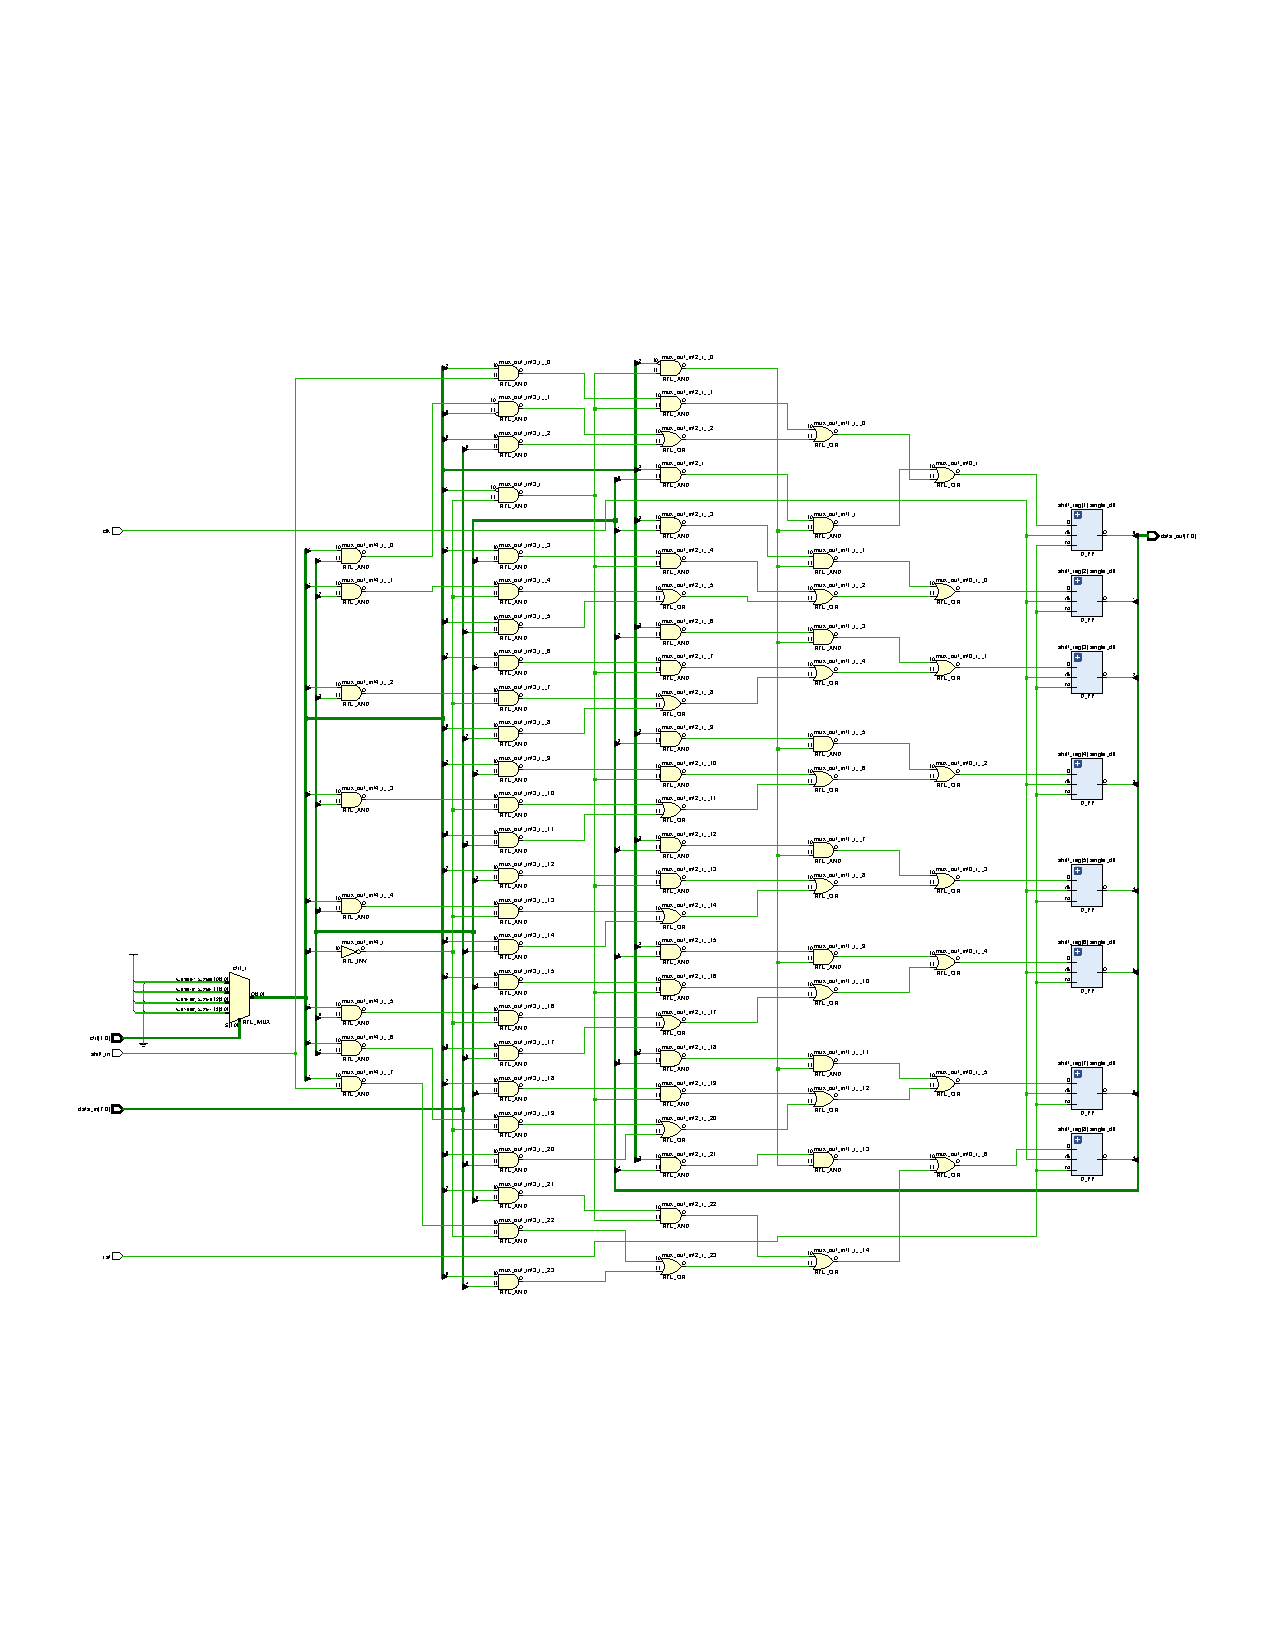
\includegraphics[width=0.95 \textwidth]{schematic_B.pdf}}
    \caption{Schematic of the parameterizable shift register}
    \label{fig:schematic_B}
\end{figure}


\newpage

\section{Conclusion}
Both of the prescribed tasks were successfully implemented and tested. This lab clearly helped one understand how to implement and test a parameterizable ALU and Shift Register in human-readable VHDL. 
\newpage



\end{document}  